% ============================================================
% Final Project Presentation
% Project 15: Document Image Machine Translation (imgtrans)
% Course: CSC15012 - Applications of NLP in Industry
% Student: Le Dinh Minh Quan - 23127460 - 23CNTThuc
% Beamer: Madrid + seahorse, aspectratio=169 (matches Project 16 style)
% Zero uploaded images: every diagram is TikZ, every chart is pgfplots.
% Only optional upload is logo_hcmus.png (guarded by \IfFileExists).
% ============================================================

\documentclass[10pt,aspectratio=169]{beamer}

\mode<presentation>
{
  \usetheme{Madrid}
  \usecolortheme{seahorse}
  \usefonttheme{default}
  \setbeamertemplate{navigation symbols}{}
  \setbeamertemplate{caption}[numbered]
  \setbeamertemplate{footline}[frame number]
}

% ---- Packages ----
\usepackage[english]{babel}
\usepackage[utf8]{inputenc}
\usepackage{amsmath}
\usepackage{amssymb}
\usepackage{graphicx}
\usepackage{booktabs}
\usepackage{xcolor}
\usepackage{hyperref}
\usepackage{xurl}
\usepackage{tikz}
\usepackage{pgfplots}
\pgfplotsset{compat=1.18}
\usetikzlibrary{shapes.geometric, arrows.meta, positioning, fit, backgrounds, shadows}
\usepackage{listings}
\lstset{
  basicstyle=\ttfamily\scriptsize,
  breaklines=true,
  frame=single,
  backgroundcolor=\color{gray!10},
  keywordstyle=\color{blue},
  commentstyle=\color{green!60!black},
  stringstyle=\color{red!70!black},
  showstringspaces=false,
  tabsize=2
}

% ---- HCMUS LOGO ----
% Upload logo_hcmus.png to Overleaf to display the logo (top-right of every slide).
% If the file is missing, no logo is shown (no error).
\IfFileExists{logo_hcmus.png}{\logo{\includegraphics[height=0.7cm]{logo_hcmus.png}}}{}

% ---- TITLE METADATA ----
\title[Project 15: Document Image MT]{Project 15: Document Image Machine Translation}
\subtitle{A layout-preserving OCR $\rightarrow$ MT $\rightarrow$ render cascade with a deterministic agent (\texttt{imgtrans})}
\author[Le Dinh Minh Quan]{Le Dinh Minh Quan \\ \small ID: 23127460 -- Class: 23CNTThuc}
\institute[HCMUS]{Vietnam National University Ho Chi Minh City \\ University of Science -- Faculty of Information Technology \\ \small Course: CSC15012 -- Applications of NLP in Industry}
\date{2026}

\begin{document}

% ============================================================
% SLIDE 1: TITLE
% ============================================================
\begin{frame}
  \titlepage
\end{frame}

% ============================================================
% SLIDE 2: OUTLINE
% ============================================================
\begin{frame}{Outline}
\begin{columns}[T]
\begin{column}{0.5\textwidth}
\begin{enumerate}
  \item Business Problem \& Motivation
  \item Proposed NLP Solution \& Success Metrics
  \item System Architecture (cascade + agent)
  \item Repository \& Tech Stack
  \item Data: the Synthetic Generator
  \item Model Selection (three slots, one trained)
  \item Training / Autopilot Workflow
  \item Evaluation Results (offline floor)
\end{enumerate}
\end{column}
\begin{column}{0.5\textwidth}
\begin{enumerate}
  \setcounter{enumi}{8}
  \item The 5-Decision Agent (D1--D5)
  \item Agent Example Traces
  \item Deployment (API / UI / Docker / Colab)
  \item Ethics, Privacy \& Fairness
  \item Monitoring \& Continual Learning
  \item Key Takeaways \& Future Work
  \item Resources \& Thank You
\end{enumerate}
\end{column}
\end{columns}
\end{frame}

% ============================================================
% SLIDE 3: BUSINESS PROBLEM & MOTIVATION
% ============================================================
\begin{frame}{1. Business Problem \& Motivation}
\begin{block}{Context}
\textbf{In-image machine translation} (the ``Google Translate camera'' experience): take an image, scan, or PDF that \emph{contains} text and produce a \emph{new image} with the text translated -- \textbf{while preserving the original layout}. Input and output are both pixels.
\end{block}

\begin{columns}[T]
\begin{column}{0.5\textwidth}
\textbf{Use cases / pain points}
\begin{itemize}\small
  \item Travel signage, menus, product labels
  \item Scanned contracts \& legal documents
  \item Forms \& official paperwork (field labels)
  \item Screenshots \& UI captures
  \item Born-digital PDFs (OCR can be bypassed)
\end{itemize}
\end{column}
\begin{column}{0.5\textwidth}
\textbf{Stakeholders}
\begin{itemize}\small
  \item Newcomers, migrants, travelers
  \item Document-localization teams (first-pass draft)
  \item Developers (REST API)
  \item Trust \& Safety / compliance (\texttt{needs\_review})
\end{itemize}
\end{column}
\end{columns}

\vspace{0.15cm}
\scriptsize The hard part is layout: translations are usually \emph{longer} than the source, so the box overflows. The user always wants \emph{the page back}, translated -- not a list of strings.
\end{frame}

% ============================================================
% SLIDE 4: PROPOSED NLP SOLUTION + SUCCESS METRICS
% ============================================================
\begin{frame}{2. Proposed NLP Solution \& Success Metrics}
\begin{block}{Solution}
A complete, license-clean \textbf{cascade} (not an end-to-end model): \textbf{OCR} (Tesseract) $\rightarrow$ \textbf{trainable MT core} (\texttt{m2m100\_418M}, fine-tuned) $\rightarrow$ \textbf{layout-preserving overlay} (Pillow), orchestrated by a deterministic \textbf{agent (D1--D5)}. Only the MT core is trained.
\end{block}

\begin{table}[h]
\centering\small
\begin{tabular}{lll}
\toprule
\textbf{Type} & \textbf{Metric} & \textbf{Target / role} \\
\midrule
Business & Layout preserved (overlay usable) & Translation anchored to original structure \\
Business & Honest degradation (no silent garbage) & Flag the hard 10\%, never fake success \\
Technical & MT quality (chrF on clean source) & Fine-tune beats all 3 baselines \\
Technical & OCR quality (CER / WER vs gold) & Quantify reading accuracy + OCR-cost gap \\
Technical & End-to-end image-translation chrF & Whole pipeline on a degraded page \\
Technical & Layout fidelity (fit-rate / shrink / overflow) & Headline deliverable; drives D5 routing \\
\bottomrule
\end{tabular}
\end{table}

\scriptsize Four metric \emph{families} isolate four failure modes; the gap \texttt{(clean MT chrF $-$ end-to-end chrF)} directly measures the cost of OCR error. A single headline number would hide which stage broke.
\end{frame}

% ============================================================
% SLIDE 5: SYSTEM ARCHITECTURE (TikZ)
% ============================================================
\begin{frame}{3. System Architecture -- Cascade + Agent (D1--D5)}
\centering
\resizebox{0.97\linewidth}{!}{%
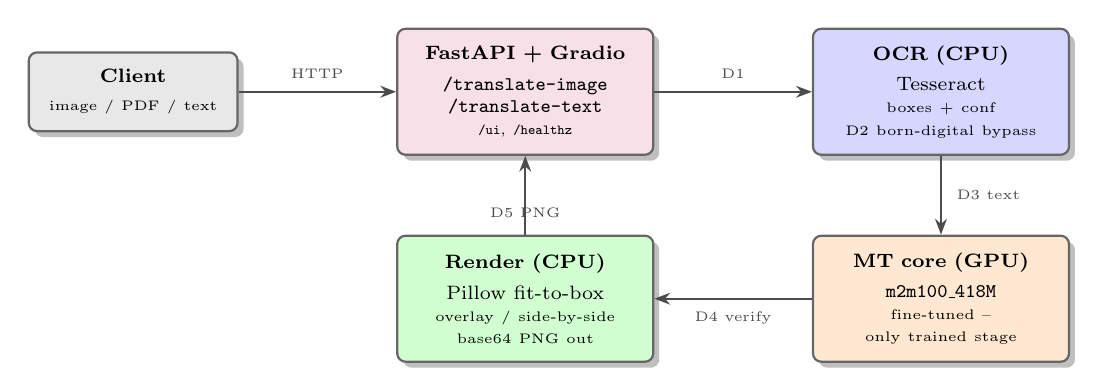
\begin{tikzpicture}[
  node distance=0.9cm and 2.0cm,
  box/.style={rectangle, draw=black!60, rounded corners=3pt, thick,
              text width=2.9cm, minimum height=1.6cm, align=center,
              inner sep=5pt, font=\scriptsize, drop shadow},
  ocrbox/.style={box, fill=blue!16},
  mtbox/.style={box, fill=orange!18},
  renderbox/.style={box, fill=green!18},
  apibox/.style={box, fill=purple!12},
  userbox/.style={box, fill=gray!18, text width=2.3cm, minimum height=1.0cm},
  arrow/.style={-{Stealth[length=2mm]}, thick, color=black!70}
]

\node[userbox] (user) {%
  \textbf{Client}\\[2pt]
  {\tiny image / PDF / text}
};
\node[apibox, right=of user] (api) {%
  \textbf{FastAPI + Gradio}\\[3pt]
  \texttt{/translate-image}\\
  \texttt{/translate-text}\\
  {\tiny \texttt{/ui}, \texttt{/healthz}}
};
\node[ocrbox, right=of api] (ocr) {%
  \textbf{OCR (CPU)}\\[3pt]
  Tesseract\\
  {\tiny boxes + conf}\\
  {\tiny D2 born-digital bypass}
};
\node[mtbox, below=1.0cm of ocr] (mt) {%
  \textbf{MT core (GPU)}\\[3pt]
  \texttt{m2m100\_418M}\\
  {\tiny fine-tuned --}\\
  {\tiny only trained stage}
};
\node[renderbox, below=1.0cm of api] (render) {%
  \textbf{Render (CPU)}\\[3pt]
  Pillow fit-to-box\\
  {\tiny overlay / side-by-side}\\
  {\tiny base64 PNG out}
};

\draw[arrow] (user) -- node[above=1pt, font=\tiny] {HTTP} (api);
\draw[arrow] (api) -- node[above=1pt, font=\tiny] {D1} (ocr);
\draw[arrow] (ocr) -- node[right=2pt, font=\tiny] {D3 text} (mt);
\draw[arrow] (mt) -- node[below=1pt, font=\tiny] {D4 verify} (render);
\draw[arrow] (render) -- node[below=1pt, font=\tiny] {D5 PNG} (api);
\end{tikzpicture}%
}

\vspace{0.15cm}
\scriptsize \textbf{Device split}: OCR (Tesseract) + render (Pillow) are CPU-only; only the MT core benefits from GPU. Every stage degrades to a deterministic stub (SeedEngine / dictionary MT / DejaVuSans) so the container always boots and \texttt{/healthz} returns ready -- even with no weights downloaded. The agent is the controller \emph{inside} the backend; the API is a thin transport layer.
\end{frame}

% ============================================================
% SLIDE 6: REPOSITORY & TECH STACK
% ============================================================
\begin{frame}[fragile]{4. Repository Structure \& Tech Stack}
\begin{columns}[T]
\begin{column}{0.55\textwidth}
\textbf{GitHub repo} (public, MIT) \\
\scriptsize \url{https://github.com/ledinhminhquan/15_Document_Image_Translation}

\vspace{0.1cm}
\begin{lstlisting}[basicstyle=\ttfamily\tiny]
15_Document_Image_Translation/
|-- src/imgtrans/
|   |-- config.py cli.py logging_utils.py
|   |-- data/      # synth_render (generator), samples
|   |-- models/    # ocr_engine (Tesseract/Seed/Stub)
|   |-- mt/         # translator (m2m100 + dictionary)
|   |-- imaging/    # layout + render (fit-to-box)
|   |-- training/   # train_mt, evaluate, metrics
|   |-- agent/      # state, policy (D1-D5), tools
|   |-- api/        # FastAPI + Gradio (/ui)
|   |-- analysis/   # error, latency, layout_fidelity
|   |-- autoreport/ # report_pdf + slides_pptx
|   |-- monitoring/ # drift_report (job-log)
|   +-- grading/    # rubric self-check
|-- configs/  docs/ (14)  notebooks/ (H100 autopilot)
|-- app/ deploy/ sample_data/ scripts/ tests/
|-- Dockerfile  docker-compose.yml  Makefile
+-- .github/workflows/ci.yml  LICENSE (MIT)  README.md
\end{lstlisting}
\end{column}
\begin{column}{0.45\textwidth}
\textbf{Tech stack} {\scriptsize(all MIT / Apache-2.0 / OFL / CC0)}
\begin{itemize}\scriptsize
  \item Python 3.11/3.12, Git + GitHub (MIT)
  \item PyTorch + HF Transformers (\texttt{Seq2SeqTrainer})
  \item \textbf{MT core (trained)}: \texttt{m2m100\_418M} (MIT, 418M, $\sim$100 langs)
  \item \textbf{OCR}: Tesseract / \texttt{pytesseract} (Apache-2.0)
  \item Born-digital router: PyMuPDF (from P07)
  \item \textbf{Render}: Pillow $\geq$ 9.2 + Noto / DejaVu
  \item Metrics: \texttt{sacrebleu} (chrF/BLEU) + pure-Python
  \item Baselines: identity, dictionary MT, zero-shot m2m100
  \item API: FastAPI + Uvicorn; UI: Gradio \texttt{Blocks} (\texttt{/ui})
  \item Docker (Tesseract + fonts + libGL); Colab H100 autopilot
  \item Optional LLM brain: \texttt{anthropic} (OFF by default)
\end{itemize}
\end{column}
\end{columns}
\end{frame}

% ============================================================
% SLIDE 7: DATA - THE SYNTHETIC GENERATOR
% ============================================================
\begin{frame}{5. Data: the Synthetic Generator (the Spine)}
\begin{columns}[T]
\begin{column}{0.52\textwidth}
\textbf{Why synthetic?}
\begin{itemize}\scriptsize
  \item Eval needs \texttt{(image, gold\_src, gold\_tgt, boxes)} quadruples
  \item \textbf{No public in-image translation benchmark exists} (datasets research returned \texttt{null})
  \item OCR sets lack translations; MT corpora lack images/layout
  \item So we \emph{do not claim} a public benchmark and \emph{do not depend} on one
\end{itemize}

\textbf{\texttt{synth\_render.py} (deterministic, per-index seeded)}
\begin{itemize}\scriptsize
  \item \texttt{rng = Random(BASE\_SEED*1\_000\_003 + i)} $\Rightarrow$ same index $\rightarrow$ same image
  \item Renders the source sentence into 1--3 blocks with the \emph{same} word-wrap as the renderer (boxes = gold layout)
  \item Mild OCR-survivable degradations: rotation $\pm3^\circ$, blur, noise, brightness/contrast, JPEG; \textbf{CLEAN mode} = OCR upper bound
\end{itemize}
\end{column}
\begin{column}{0.48\textwidth}
\textbf{Sources \& licenses} {\scriptsize(non-commercial = FLAGGED)}
\begin{table}[h]
\centering\scriptsize
\begin{tabular}{lll}
\toprule
\textbf{Source} & \textbf{License} & \textbf{Role} \\
\midrule
\texttt{synth\_render} & ours & PRIMARY \\
\texttt{opus-100} en-fr & unknown & \textbf{FLAG} \\
Post-OCR-Correction & CC0 & optional \\
Seed pages + dict & ours & offline \\
Noto Sans & OFL 1.1 & glyphs \\
DejaVuSans & bundled & fallback \\
\bottomrule
\end{tabular}
\end{table}
\scriptsize \textbf{Splits}: MT train up to $\sim$1M pairs; MT test (clean) a few k; image eval 200--2000 quadruples + a CLEAN twin (matched content $\rightarrow$ exact OCR-cost gap); 3--5 committed fixture PNGs.

\vspace{0.05cm}
\scriptsize \textbf{Never shipped}: \texttt{nllb-200-distilled-600M} (CC-BY-NC) and Surya (CC-BY-NC-SA) -- research-only.
\end{column}
\end{columns}
\end{frame}

% ============================================================
% SLIDE 8: MODEL SELECTION
% ============================================================
\begin{frame}{6. Model Selection -- Three Slots, One Trained}
\begin{columns}[T]
\begin{column}{0.5\textwidth}
\textbf{The three pipeline slots}
\begin{table}[h]
\centering\scriptsize
\begin{tabular}{lll}
\toprule
\textbf{Slot} & \textbf{Trained?} & \textbf{Default} \\
\midrule
MT core & \textbf{YES} & \texttt{m2m100\_418M} (MIT) \\
OCR & no & Tesseract (Apache) \\
Render & no & Pillow fit-to-box \\
\bottomrule
\end{tabular}
\end{table}

\textbf{Why \texttt{m2m100\_418M}}
\begin{itemize}\scriptsize
  \item License decisive: \textbf{MIT}, fully permissive (NLLB is better but CC-BY-NC $\Rightarrow$ rejected)
  \item Many-to-many $\Rightarrow$ \textbf{one checkpoint} serves en$\rightarrow$fr \emph{and} multilingual (direction is a runtime arg)
  \item 418M fits the free-Colab T4 floor (fp16 + grad-accum)
  \item Reuses the P13/P14 \texttt{Seq2SeqTrainer} harness verbatim
\end{itemize}
\end{column}
\begin{column}{0.5\textwidth}
\textbf{Why Tesseract; why not end-to-end VLM}
\begin{itemize}\scriptsize
  \item \texttt{image\_to\_data} fuses detection + recognition + \emph{confidence} in one call -- no detector to train
  \item A VLM (\texttt{GOT-OCR-2.0}, \texttt{pix2struct}) \emph{reads} but discards the geometry the overlay needs
  \item The cascade \textbf{exposes} the signals the agent gates on (conf, coverage, round-trip, fit) a black box hides
\end{itemize}

\textbf{Render: pure Pillow (no neural inpaint)}
\begin{itemize}\scriptsize
  \item Erase = algorithmic whiteout (2px border-ring median)
  \item Fit-to-box = binary search over font size + greedy word-wrap (per-char for CJK) $\rightarrow$ \texttt{fit\_ok}
  \item Erase-all-then-draw ordering; Noto by script + DejaVu fallback
\end{itemize}

\textbf{Baselines}: identity (floor), dictionary MT (= offline engine), zero-shot m2m100 (what fine-tuning buys).
\end{column}
\end{columns}
\end{frame}

% ============================================================
% SLIDE 9: TRAINING / AUTOPILOT WORKFLOW (TikZ)
% ============================================================
\begin{frame}{7. Training / Autopilot Workflow -- H100 Notebook}
\centering
\begin{tikzpicture}[
  node distance=0.16cm,
  step/.style={rectangle, draw=black!60, rounded corners=2pt, thick,
              minimum width=11.6cm, minimum height=0.55cm, align=center, font=\scriptsize},
  setup/.style={step, fill=gray!15},
  train/.style={step, fill=orange!15},
  eval/.style={step, fill=blue!15},
  deploy/.style={step, fill=green!15},
  arrow/.style={-{Stealth[length=1.8mm]}, thick}
]
\node[setup] (s1) {\textbf{1. Setup (Colab)}: install Tesseract + Noto fonts, clone repo, set \texttt{ARTIFACTS\_DIR} on Drive};
\node[setup, below=of s1] (s2) {\textbf{2. Data}: load \texttt{opus-100} en-fr; \texttt{synth\_render.py} builds \texttt{(image, gold\_src, gold\_tgt, boxes)} (200--2000)};
\node[train, below=of s2] (s3) {\textbf{3. MT fine-tune}: \texttt{m2m100\_418M} via HF \texttt{Seq2SeqTrainer} (fp16, resume-safe), headline metric chrF};
\node[eval, below=of s3] (s4) {\textbf{4. MT eval}: fine-tuned vs baselines (identity, dictionary, zero-shot) on held-out opus-100};
\node[eval, below=of s4] (s5) {\textbf{5. OCR eval}: Tesseract CER/WER vs gold source on CLEAN + degraded synthetic pages};
\node[eval, below=of s5] (s6) {\textbf{6. End-to-end + layout}: \texttt{MT(OCR(image))} chrF; fit-rate / mean-shrink / overflow; OCR-cost gap};
\node[deploy, below=of s6] (s7) {\textbf{7. Auto-gen} report PDF (\texttt{reportlab}) + slides PPTX (\texttt{python-pptx})};
\node[deploy, below=of s7] (s8) {\textbf{8. Grade \& bundle}: rubric self-check (\texttt{grading/checklist.py}) + submission bundle to Drive};
\foreach \a/\b in {s1/s2,s2/s3,s3/s4,s4/s5,s5/s6,s6/s7,s7/s8}
  \draw[arrow] (\a) -- (\b);
\end{tikzpicture}

\vspace{0.12cm}
\scriptsize \textbf{One-button Run-All} on Colab H100 (auto-adapts A100/L4/T4). The fine-tune step is resume-safe against disconnects. Capability probes upgrade each stage to the real backend when present, so the \emph{same code path} runs offline (CPU) and online (GPU). \texttt{P15\_OFFLINE=1} pins stub mode for reproducible CI.
\end{frame}

% ============================================================
% SLIDE 10: EVALUATION RESULTS + pgfplots chart
% ============================================================
\begin{frame}{8. Evaluation Results -- Verified Offline Seed Floor}
\begin{columns}[T]
\begin{column}{0.54\textwidth}
\textbf{Offline seed evaluation} {\scriptsize(stdlib + Pillow only)}
\begin{table}[h]
\centering\scriptsize
\begin{tabular}{llc}
\toprule
\textbf{Metric} & \textbf{Family} & \textbf{Value} \\
\midrule
MT chrF (dictionary) & MT quality & \textbf{79.9} \\
MT chrF (identity floor) & MT quality & 22.4 \\
OCR CER & OCR quality & \textbf{0.0} \\
End-to-end chrF & End-to-end & \textbf{76.4} \\
Mean fit-rate & Layout & \textbf{1.0} \\
\bottomrule
\end{tabular}
\end{table}
\scriptsize Self-check grade \textbf{0.97}; all \textbf{5 decision points fire}; \textbf{22 tests pass} (CPU-only, no downloads). OCR-cost gap $= 79.9 - 76.4 = \mathbf{3.5}$ chrF.

\vspace{0.1cm}
\footnotesize \textbf{Read honestly}: dictionary chrF \emph{saturates} on the seed because seed pairs overlap the glossary -- an \emph{artifact, not a result}. On real held-out \texttt{opus-100} pairs the \textbf{fine-tuned m2m100 dominates}; that non-saturated story is produced by the real Colab H100 run. OCR CER 0.0 is a \emph{ceiling} (SeedEngine reads gold), and fit-rate 1.0 is \emph{by construction} on synthetic.
\end{column}
\begin{column}{0.46\textwidth}
\centering
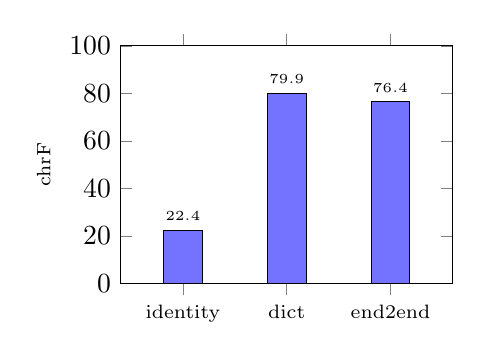
\begin{tikzpicture}
\begin{axis}[
  ybar, width=5.8cm, height=4.6cm,
  ymin=0, ymax=100,
  symbolic x coords={identity, dict, end2end},
  xtick=data,
  x tick label style={font=\scriptsize},
  ylabel={chrF},
  ylabel style={font=\scriptsize},
  nodes near coords, nodes near coords style={font=\tiny},
  bar width=14pt,
  enlarge x limits=0.3,
  ytick={0,20,40,60,80,100}
]
\addplot[fill=blue!55] coordinates {(identity,22.4) (dict,79.9) (end2end,76.4)};
\end{axis}
\end{tikzpicture}\\
{\tiny chrF: identity floor vs dictionary MT vs end-to-end \texttt{MT(OCR(image))}.}

\vspace{0.1cm}
{\scriptsize \textbf{Layout fidelity} on synthetic: mean fit-rate $=$ \textbf{1.0}, mean shrink $=$ 1.0, overflow $=$ 0 -- every block fit its box. On real photos fit-rate falls and the D5 side-by-side branch fires (the designed-for common case).}
\end{column}
\end{columns}
\end{frame}

% ============================================================
% SLIDE 11: THE 5-DECISION AGENT (TikZ pipeline)
% ============================================================
\begin{frame}{9. The 5-Decision Agent (Deterministic FSM)}
\centering
\resizebox{0.97\linewidth}{!}{%
\begin{tikzpicture}[
  node distance=0.22cm,
  step/.style={rectangle, draw=black!60, rounded corners=2pt, thick,
              text width=12.6cm, inner sep=4pt, minimum height=0.6cm,
              align=center, font=\scriptsize},
  ingest/.style={step, fill=gray!15},
  ocr/.style={step, fill=blue!15},
  trans/.style={step, fill=orange!15},
  verify/.style={step, fill=purple!15},
  render/.style={step, fill=green!15},
  arrow/.style={-{Stealth[length=2mm]}, thick}
]
\node[ingest] (d1) {\textbf{D1 -- INGEST}: image $\rightarrow$ OCR; pdf $\rightarrow$ D2; \texttt{.txt} $\rightarrow$ skip OCR (jump to D4); unsupported $\rightarrow$ \texttt{needs\_review}};
\node[ocr, below=of d1] (d2) {\textbf{D2 -- OCR (PDF)}: PyMuPDF coverage $\geq$ thr $\rightarrow$ \textbf{use text layer, BYPASS OCR} (zero OCR error); else rasterize $\rightarrow$ Tesseract};
\node[trans, below=of d2] (d3) {\textbf{D3 -- TRANSLATE}: conf $\geq$ 75 $\rightarrow$ MT; 40--75 $\rightarrow$ re-OCR (gamma/upscale/invert); $<$40 or garbage $\rightarrow$ drop + \texttt{needs\_review}};
\node[verify, below=of d3] (d4) {\textbf{D4 -- VERIFY}: round-trip chrF $\geq \tau$ AND length ratio $\in [0.4,3.0]$ $\rightarrow$ accept; rt $< \tau$ $\rightarrow$ re-decode once $\rightarrow$ else \texttt{low\_confidence}};
\node[render, below=of d4] (d5) {\textbf{D5 -- RENDER}: \texttt{fit\_ok} at $\geq$ min font $\rightarrow$ \textbf{OVERLAY}; too long $\rightarrow$ \textbf{SIDE\_BY\_SIDE}; fit fails / D3-D4 flagged $\rightarrow$ \texttt{needs\_review}};
\foreach \a/\b in {d1/d2,d2/d3,d3/d4,d4/d5}
  \draw[arrow] (\a) -- (\b);
\end{tikzpicture}%
}

\vspace{0.1cm}
\scriptsize \textbf{Deterministic} (same input + config $\rightarrow$ byte-identical output), \textbf{fail-soft} (every point has a degrade branch), \textbf{self-checking without a reference} (D4 uses the model's own back-translation). Each state records a \texttt{ToolTrace} entry (step, branch, signal, threshold, tool, block id) so every run is auditable. The only back-edges are bounded single-shot retries in D3/D4 $\Rightarrow$ the FSM always terminates. Optional LLM brain is OFF by default, \textbf{advisory only} -- never rewrites, never overrides a branch.
\end{frame}

% ============================================================
% SLIDE 12: AGENT DECISION TABLE + EXAMPLE TRACES
% ============================================================
\begin{frame}[fragile]{10. Agent: Decision Table \& Example Traces}
\begin{table}[h]
\centering\scriptsize
\setlength{\tabcolsep}{3pt}
\begin{tabular}{llll}
\toprule
\textbf{Point} & \textbf{Intermediate signal} & \textbf{Threshold} & \textbf{Accept / degrade / fail} \\
\midrule
D1 & MIME + magic-bytes + ext & \texttt{supported\_exts} & image/pdf/text route; else \texttt{needs\_review} \\
D2 & PyMuPDF text coverage & \texttt{born\_digital\_ratio} & $\geq$ thr $\rightarrow$ bypass OCR; else rasterize \\
D3 & block mean conf + char sanity & high$\approx$75, low$\approx$40 & MT / re-OCR / drop + \texttt{needs\_review} \\
D4 & round-trip chrF; length ratio & $\tau\approx$0.45; $[0.4,3.0]$ & accept / re-decode / \texttt{low\_confidence} \\
D5 & \texttt{fit\_ok} + D4 ratio & \texttt{font\_size\_min} & OVERLAY / SIDE\_BY\_SIDE / \texttt{needs\_review} \\
\bottomrule
\end{tabular}
\end{table}

\begin{lstlisting}[basicstyle=\ttfamily\tiny]
# Example 1 -- Clean English page -> OVERLAY
  D1 ingest : input_kind=image -> OCR path (D2 no-op)
  D3 ocr    : block conf=91.3 >= 75 -> accept, send to MT
  D4 verify : round_trip_chrf=83.7, length_ratio=1.18 -> accept
  D5 render : fit_ok=true at font_size=28 -> OVERLAY
Output: render_mode=overlay, needs_review=false, layout={fit_rate:1.0, overflow:0}

# Example 2 -- Long FR translation overflows -> SIDE_BY_SIDE
  D4 verify : length_ratio=2.6 (in band) but long -> forward ratio to D5
  D5 render : fit_ok=false at font_size_min -> SIDE_BY_SIDE (expected en->fr expansion)

# Example 3 -- Unreadable smudged block -> needs_review
  D3 ocr    : block conf=31 < low(40) -> DROP block (never translate garbage)
  D5 render : block D3-flagged -> needs_review (boxes + raw text, no destructive render)
\end{lstlisting}
\end{frame}

% ============================================================
% SLIDE 13: DEPLOYMENT
% ============================================================
\begin{frame}[fragile]{11. Deployment -- API / UI / Docker / Colab}
\textbf{Four deployment formats} {\scriptsize(deployable, but \emph{not} hosted at a live public URL -- the deliverable is the capability)}
\begin{columns}[T]
\begin{column}{0.52\textwidth}
\begin{itemize}\scriptsize
  \item \textbf{REST API} (FastAPI): \texttt{GET /healthz}, \texttt{GET /version}, \texttt{POST /translate-text}, \texttt{POST /translate-image}
  \item \textbf{CLI}: \texttt{imgtrans serve / demo-agent / translate-text / translate-image / evaluate / autopilot}
  \item \textbf{Gradio demo UI}: \texttt{Blocks} mounted at \texttt{/ui} (one process, one port serves API + demo)
  \item \textbf{Docker}: Tesseract + Noto/DejaVu + libGL baked in; plus a one-button Colab H100 autopilot
\end{itemize}
\end{column}
\begin{column}{0.48\textwidth}
\begin{table}[h]
\centering\scriptsize
\begin{tabular}{ll}
\toprule
\textbf{Endpoint} & \textbf{Behaviour} \\
\midrule
\texttt{/healthz} & readiness + resolved config \\
\texttt{/translate-text} & text-in/out (skips OCR+render) \\
\texttt{/translate-image} & full cascade $\rightarrow$ overlay PNG \\
\bottomrule
\end{tabular}
\end{table}
\scriptsize \textbf{Error contract}: \texttt{200} even for \texttt{needs\_review:true} (defensible result, not an error); \texttt{400} unsupported type (D1); \texttt{413} oversized; \texttt{415} upload route off; \texttt{422} validation.
\end{column}
\end{columns}

\vspace{0.1cm}
\scriptsize \textbf{Device}: OCR + render CPU-only; only MT benefits from GPU. \texttt{P15\_DEVICE=auto} $\rightarrow$ \texttt{cuda} else \texttt{cpu}. Latency dominated by MT decode then OCR; render is sub-10\,ms/block; D2 born-digital bypass is the fastest path (zero OCR error); \texttt{verify=true} (D4) doubles MT decode and can be disabled for batch throughput. 12-factor config via \texttt{P15\_*} env vars, readable in \texttt{/healthz}; \texttt{P15\_MT\_MODEL} must never be a non-commercial id in production.
\end{frame}

% ============================================================
% SLIDE 14: ETHICS, PRIVACY & FAIRNESS
% ============================================================
\begin{frame}{12. Ethics, Privacy \& Bias}
\begin{columns}[T]
\begin{column}{0.5\textwidth}
\textbf{Privacy} {\scriptsize(document images = highly sensitive PII)}
\begin{itemize}\scriptsize
  \item \textbf{Local / on-device by default}: no network egress at inference (download only at setup)
  \item \textbf{No raw-image retention}: \texttt{/translate-image} processes in memory, persists nothing
  \item LLM brain OFF $\Rightarrow$ no document text/image leaves the machine
  \item Minimisation: block-level processing; D3 drops low-conf blocks (never stores them)
\end{itemize}

\textbf{The tool assists, it does not decide}
\begin{itemize}\scriptsize
  \item Three lossy stages stacked $\Rightarrow$ errors propagate; output \emph{looks} authoritative
  \item D3 never translates garbage; D4 catches hallucination/truncation; D5 degrades instead of faking
  \item A competent human must review before reliance (legal/medical)
\end{itemize}
\end{column}
\begin{column}{0.5\textwidth}
\textbf{Bias -- measure and disclose, not claim removed}
\begin{itemize}\scriptsize
  \item \textbf{MT bias}: gendered target languages force gender; dialects/registers translate worse; m2m100 uneven across $\sim$100 langs
  \item \textbf{OCR bias}: Tesseract strongest on Latin print, weaker on Arabic/Devanagari/Thai, CJK, handwriting $\Rightarrow$ a less-supported script enters MT more corrupted
  \item Metrics reported \textbf{per language pair and per condition} -- never one headline number that hides disparity
\end{itemize}

\textbf{Licensing as an ethical choice}
\begin{itemize}\scriptsize
  \item Ship only MIT / Apache-2.0 / OFL / CC0
  \item NLLB (CC-BY-NC) + Surya (CC-BY-NC-SA) flagged, never shipped; verify each opus-100 pair
\end{itemize}
\end{column}
\end{columns}

\vspace{0.08cm}
\scriptsize \emph{One-line ethic}: translate what it can read, flag what it cannot, never assert certainty, keep the original for a human.
\end{frame}

% ============================================================
% SLIDE 15: MONITORING & CONTINUAL LEARNING
% ============================================================
\begin{frame}{13. Monitoring \& Continual Learning}
\begin{columns}[T]
\begin{column}{0.52\textwidth}
\textbf{Monitoring}: one model to retrain, three quality surfaces to watch
\begin{table}[h]
\centering\scriptsize
\begin{tabular}{ll}
\toprule
\textbf{Surface} & \textbf{Signal (decision)} \\
\midrule
Routing health & D1 / D5 final route \\
OCR quality & D3 conf; D2 router \\
Translation quality & D4 round-trip + ratio \\
Layout fidelity & D5 \texttt{fit\_box} \\
Latency / cost & per-stage timing \\
\bottomrule
\end{tabular}
\end{table}
\scriptsize Each request appends one \textbf{metrics-only} JSONL row (\texttt{runs/serve/jobs-*.jsonl}); no raw image/text by default. Drift = threshold drift on scalars + distribution drift (PSI $>$ 0.2) on length-ratio / round-trip / OCR-conf. \textbf{OCR drift and MT drift attributed separately} (OCR is not retrained by us); the born-digital-bypass slice gives a clean OCR-free MT signal.
\end{column}
\begin{column}{0.48\textwidth}
\textbf{Continual learning} (target is \emph{always and only} m2m100)
\begin{enumerate}\scriptsize
  \item Capture feedback on \texttt{side\_by\_side} / \texttt{needs\_review} (the informative tail)
  \item Reviewer verdict (\texttt{ocr\_wrong} / \texttt{mt\_wrong} / \texttt{both} / \texttt{acceptable}) routes the fix: \texttt{mt\_wrong} $\rightarrow$ parallel pair; \texttt{ocr\_wrong} $\rightarrow$ OCR-robustness pair (translate \emph{through} the noise)
  \item \texttt{curate.py}: PII scrub + consent + dedup + sanity + agreement
  \item Re-fine-tune m2m100 with the same \texttt{Seq2SeqTrainer}
  \item Promote \textbf{only if} champion--challenger gate passes (end-to-end chrF up, clean MT not regressed, needs-review not up)
\end{enumerate}
\scriptsize Promotion bumps \texttt{model\_version} + resets the drift baseline; non-commercial NLLB/Surya hard-blocked from any promoted checkpoint.
\end{column}
\end{columns}
\end{frame}

% ============================================================
% SLIDE 16: KEY TAKEAWAYS & FUTURE WORK
% ============================================================
\begin{frame}{14. Key Takeaways \& Future Work}
\textbf{Key takeaways}
\begin{itemize}\small
  \item A complete, license-clean in-image translation \textbf{cascade} (OCR $\rightarrow$ MT $\rightarrow$ layout-preserving render); \texttt{m2m100\_418M} (MIT) is the \emph{single} trained stage
  \item A deterministic \textbf{5-decision agent (D1--D5)} with a self-checking degradation ladder (\texttt{overlay} $\rightarrow$ \texttt{side\_by\_side} $\rightarrow$ \texttt{needs\_review}) -- a defensible output on every input
  \item A reproducible \textbf{synthetic generator} that constructs the \texttt{(image, gold\_src, gold\_tgt, boxes)} quadruples no public benchmark provides $\Rightarrow$ four exact metric families
  \item Verified offline floor: dictionary chrF \textbf{79.9} vs identity \textbf{22.4}, OCR CER \textbf{0.0}, end-to-end chrF \textbf{76.4}, fit-rate \textbf{1.0}, grade \textbf{0.97}, all 5 decisions fire, 22 tests pass -- the honest non-saturated quality story lives on the real Colab H100 run
  \item Deployable as REST API + Gradio UI + Docker + one-button Colab H100 autopilot; every shipped component MIT / Apache-2.0 / OFL / CC0
\end{itemize}

\textbf{Future work}
\begin{enumerate}\small
  \item A real held-out, \texttt{hub\_repo\_details}-verified in-image benchmark, wired as a test split
  \item H100 quality upgrades: \texttt{mbart-large-50-mmt} (MIT), \texttt{trocr-large-printed} / \texttt{GOT-OCR-2.0-hf} for tough photos
  \item Better erase (simple-inpaint smear + blur on textured backgrounds), short of a neural inpainter
  \item Full RTL shaping (\texttt{python-bidi} + \texttt{arabic-reshaper}) instead of best-effort logical order
  \item Real-time drift dashboard over the JSONL job logs + automated champion--challenger retrain
\end{enumerate}
\end{frame}

% ============================================================
% SLIDE 17: RESOURCES & THANK YOU (Final slide)
% ============================================================
\begin{frame}{15. Resources \& Thank You}
\begin{block}{Source code (public, MIT)}
\centering
\large \textbf{\url{https://github.com/ledinhminhquan/15_Document_Image_Translation}}
\end{block}

\textbf{What ships in the repo}
\begin{itemize}\scriptsize
  \item \textbf{Package} \texttt{imgtrans}: OCR / MT / imaging+render / agent (D1--D5) / API / analysis / autoreport / monitoring / automation / grading
  \item \textbf{14 rubric-aligned docs} under \texttt{docs/} (+ \texttt{DESIGN\_BRIEF.md}); a one-button \textbf{H100 autopilot notebook} + \texttt{COLAB\_GUIDE.md}
  \item \textbf{Deployable surface}: FastAPI REST API + Gradio demo UI (mounted at \texttt{/ui}) + Docker image (Tesseract + Noto/DejaVu + libGL) + Colab H100 autopilot
  \item \textbf{Offline test path}: \texttt{pytest -q} runs \texttt{image $\rightarrow$ OCR(SeedEngine) $\rightarrow$ MT(dictionary) $\rightarrow$ render(DejaVu) $\rightarrow$ all metrics} with no downloads (\texttt{HF\_HUB\_OFFLINE})
\end{itemize}

\scriptsize \emph{Note}: the system is \textbf{deployable} but is \emph{not} currently hosted at a live public URL; the deliverable is the API / UI / Docker / Colab capability above. Every shipped component is MIT / Apache-2.0 / OFL / CC0; non-commercial options (NLLB, Surya) are flagged and never shipped.

\vspace{0.25cm}
\centering
\Large\textbf{Thank you for your attention!}\\[0.2cm]
\normalsize Le Dinh Minh Quan -- 23127460 -- 23CNTThuc \\
\small CSC15012 -- Applications of NLP in Industry -- 2026
\end{frame}

\end{document}
